\section{Types de services Cloud}
La plupart des services de cloud computing peuvent être classés en trois grandes catégories : IaaS (infrastructure as a service), PaaS (platform as a service), SaaS (software as a service). On les appelle parfois « pile » de cloud computing, car elles s’empilent les unes sur les autres. Si vous savez en quoi elles consistent et en quoi elles sont différentes, vous pourrez plus facilement atteindre vos objectifs.
Ses derniers temps se rajoute a ses 3 services deux autres qu'on va présenter ci-dessous.

\begin{figure}[h]
	\centering
	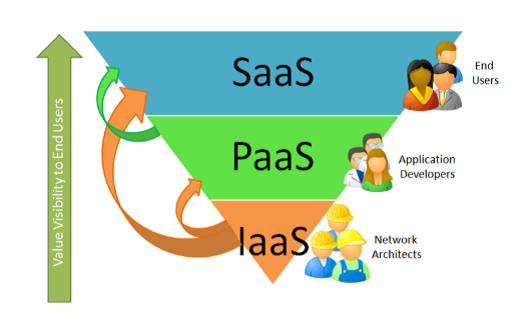
\includegraphics[scale=0.7]{img/2.4}
	\caption{Services cloud}
\end{figure}

\begin{tabular}{|p{3cm}|p{6cm}|p{5cm}|} \hline
%1ere ligne
\textbf{Service}
& \textbf{Définition}
& \textbf{Exemple} \\ \hline

%2eme ligne
\begin{center}
Infrastructure as a service (IaaS)
\end{center} 
& 
La catégorie la plus basique des services de cloud computing. Avec l’IaaS, vous louez une infrastructure informatique (serveurs, machines virtuelles, stockage, réseaux, systèmes d’exploitation) auprès d’un fournisseur de services cloud, avec un paiement en fonction de l’utilisation.
& 
\begin{itemize}[label=\textbullet]
\item Amazon EC2 Elastic Compute Cloud.
\item S3 / Simple Storage Service d'Amazon.
\item Google drive, DropBox qui sont gratuits.
\end{itemize} 
\\ \hline

%3eme ligne
\begin{center}
Platform as a service (PaaS)  
\end{center}
& 
L’expression plateforme en tant que service (PaaS, Platform-as-a-Service) qualifie les services de cloud computing qui offrent un environnement à la demande pour développer, tester, fournir et gérer des applications logicielles. PaaS est conçu pour permettre aux développeurs de créer rapidement des applications web ou mobiles sans avoir à se préoccuper de la configuration ou de la gestion de l’infrastructure de serveurs, de stockage, de réseau et de bases de données nécessaire au développement. 
& 
\begin{itemize}[label=\textbullet]
\item App Engine de Google qui se limite à Java et Python.
\item Windows Azure de Microsoft permet de travailler avec les langages comme .NET, PHP, Python, Ruby et Java.
\end{itemize} 
\\ \hline
\end{tabular}

\begin{table}
\begin{tabular}{|p{3cm}|p{6cm}|p{5cm}|} \hline
%4ere ligne
\begin{center}
Software as a service (SaaS)  
\end{center}
& 
Le logiciel en tant que service (SaaS, Software-as-a-Service) est une méthode de diffusion d’applications logicielles via Internet, à la demande et en général sur abonnement. Avec le SaaS, les fournisseurs de services cloud hébergent et gèrent les applications logicielles et l’infrastructure sous-jacente, et gèrent la maintenance, par exemple la mise à niveau des logiciels et l’application des correctifs de sécurité. Les utilisateurs se connectent à l’application via Internet, en général par l’intermédiaire d’un navigateur web sur leur téléphone, leur tablette. 
& 
\begin{itemize}[label=\textbullet]
\item Google apps avec Google Docs, Calendar et Gmail qui sont gratuites.
\item Facebook, Linkdin qui sont gratuits.
\item Offices 365 de Microsoft propose des applications web (Word,Excel, PowerPoint, Publisher...).
\end{itemize} 
\\ \hline

%4ere ligne
\begin{center}
DBaaS (DataBase as a service ) 
\end{center}
& 
Un tel modèle fournit des mécanismes transparents pour créer, stocker, accéder et mettre à jour des bases de données. De plus, le fournisseur de services de base de données assume l'entière responsabilité de l'administration de la base de données, garantissant ainsi la sauvegarde, la réorganisation et les mises à jour de version. L'utilisation de ce service permet aux fournisseurs de répliquer et de personnaliser leurs données sur plusieurs serveurs, qui peuvent être physiquement séparé [16].
& 
\begin{itemize}[label=\textbullet]
\item Amazon Web Services.
\item RackSpace.
\item IBM, Microsoft, Oracle.
\end{itemize} 
\\ \hline

%4ere ligne
\begin{center}
Informatique serverless 
\end{center}
& 
Se chevauchant avec PaaS, l’informatique Serverless se concentre sur la création de fonctionnalités applicatives sans perte de temps en lien avec la gestion permanente des serveurs et de l’infrastructure requise à cette fin. Le fournisseur de cloud se charge de la configuration, de la planification de la capacité et de l’administration du serveur à votre place. Les architectures serverless sont hautement scalables et basées sur des événements. Elle n’utilisent des ressources que quand une fonction ou un déclencheur spécifiques s’activent.
& 
\begin{itemize}[label=\textbullet]
\item Google apps avec Google Docs, Calendar et Gmail qui sont gratuites.
\item Facebook, Linkdin qui sont gratuits.
\item Offices 365 de Microsoft propose des applications web (Word,Excel, PowerPoint, Publisher...).
\end{itemize} 
\\ \hline
\end{tabular}
\caption{Les services Cloud}
\end{table}